\documentclass[runningheads]{llncs}
\usepackage{xcolor}
\usepackage{url}
\usepackage{graphicx} 
\usepackage{amssymb}
\usepackage{amsmath}
\usepackage{tikz}
\usetikzlibrary{arrows.meta, positioning, fit}

\definecolor{uf_blue}{RGB}{17,27, 150}
\definecolor{uf_orange}{RGB}{150,100,17}

\begin{document}

\title{Learning to Dispatch: A Reinforcement Learning Framework for Train Networks}

\author{\textcolor{uf_blue}{Andres Espinosa}}
\institute{
    \textcolor{uf_orange}{Industrial and Systems Engineering \\
    University of Florida}\\
    \textcolor{uf_orange}{\email{andresespinosa@ufl.edu}}
}
\maketitle


\begin{abstract}

\end{abstract}



\section{Introduction}
\label{sse:introduction}

\section{Problem Background}
\label{sse:background}
\subsection{Train Dispatch Problem}
\label{sss:train}
% This should cover the MIP formulation and the general outline of the problem
% This should also cover the DISPLIB data format and all that.
\subsection{Deep Reinforcement Learning}
\label{sss:reinforcement_learning}
% Cover Markov Decision Processes
% As well as DQN
\subsubsection{Markov Decision Processes}



\begin{figure}
    \centering
    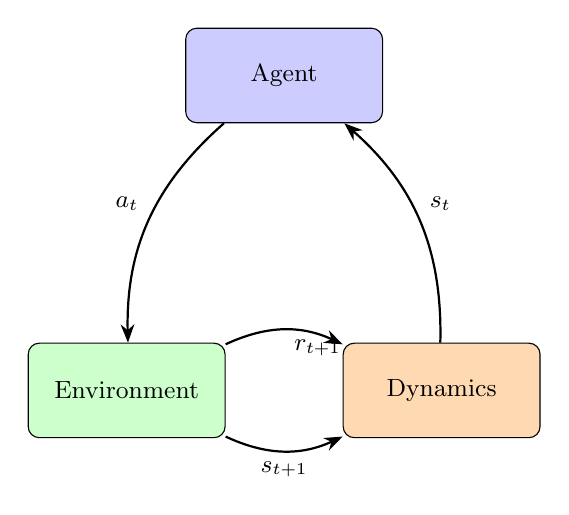
\begin{tikzpicture}[
      agent/.style={draw, rounded corners, fill=blue!20, minimum width=2.5cm, minimum height=1.2cm},
      env/.style={draw, rounded corners, fill=green!20, minimum width=2.5cm, minimum height=1.2cm},
      reward/.style={draw, rounded corners, fill=orange!30, minimum width=2.5cm, minimum height=1.2cm},
      arrow/.style={->, thick, >=Stealth},
      every node/.style={font=\small}
      ]
    
    % Nodes
    \node[agent] (agent) at (0, 2) {Agent};
    \node[env] (env) at (-2, -2) {Environment};
    \node[reward] (reward) at (2, -2) {Dynamics};
    
    % Arrows
    \draw[arrow] (agent) to[bend right=25] node[above left] {$a_t$} (env);
    \draw[arrow] (env) to[bend right=25] node[below] {$s_{t+1}$} (reward);
    \draw[arrow] (reward) to[bend right=25] node[above right] {$s_t$} (agent);
    \draw[arrow] (env) to[bend left=25] node[below right] {$r_{t+1}$} (reward);
    
    \end{tikzpicture}
    \caption{The reinforcement learning framework.}
    \label{fig:rl_framework}
\end{figure}

\subsubsection{Deep Q-Network}


\begin{figure}
    \centering
    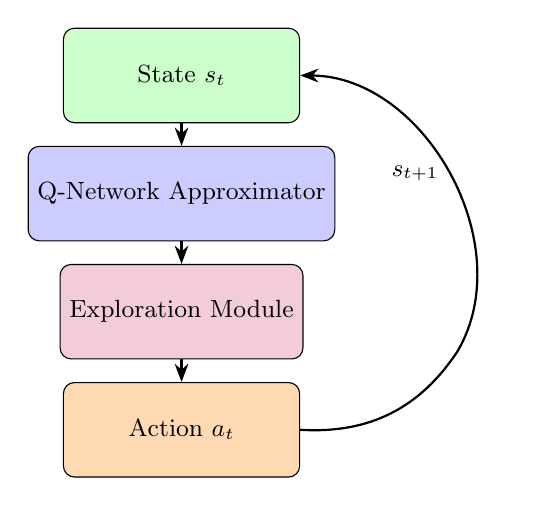
\begin{tikzpicture}[
      qnet/.style={draw, rounded corners, fill=blue!20, minimum width=3cm, minimum height=1.2cm},
      module/.style={draw, rounded corners, fill=purple!20, minimum width=3cm, minimum height=1.2cm},
      action/.style={draw, rounded corners, fill=orange!30, minimum width=3cm, minimum height=1.2cm},
      state/.style={draw, rounded corners, fill=green!20, minimum width=3cm, minimum height=1.2cm},
      arrow/.style={->, thick, >=Stealth},
      every node/.style={font=\small}
    ]
    
    % Nodes
    \node[state] (state) at (0, 2) {State $s_t$};
    \node[qnet] (qnet) at (0, 0.5) {Q-Network Approximator};
    \node[module] (explore) at (0, -1) {Exploration Module};
    \node[action] (action) at (0, -2.5) {Action $a_t$};
    
    % Arrows
    \draw[arrow] (state) -- (qnet);
    \draw[arrow] (qnet) -- (explore);
    \draw[arrow] (explore) -- (action);
    \draw[arrow] (action.east) to[bend right=30] node[right] {} ++(2,1) 
        to[bend right=60] node[left] {$s_{t+1}$} (state.east);

    \end{tikzpicture}
    \caption{The Deep Q-Network action selection and feedback loop.}
    \label{fig:dqn_loop}
\end{figure}



\subsection{Graph Neural Networks}
\label{sss:gnn}
% Cover graph neural networks

\section{Related Work}
\label{sse:related_work}
% This can be a full literature review following the structure of:
% 1) Train Dispatch Problem Formulation
% 2) Deep Reinforcement Learning with similar problems
% 3) Graph Neural Networks
I am \cite{gnndrl:Devailly_2022}
\section{Formulation}
\label{sse:formulation}

\subsection{Train Operation Graphs}
\label{sss:train_ops}


\subsection{Resource Conflict Graphs}
\label{sss:resource_conflicts}


\subsection{State Space}
\label{sss:state_space}

\subsection{Action Space}
\label{sss:action_space}

\section{Preliminary Agent Results}
\label{sse:results}

\subsection{Deep Graph Q-Network Agent}
\label{sss:agent}


\subsection{Solutions}
\label{sss:solutions}


\section{Conclusion and Future Work}
\label{sse:conclusion}

\subsection{Future Work}
\label{sss:future_work}

\subsection{Conclusion}
\label{sss:conclusion}


\section{Appendix}

\begin{figure}
    \centering
    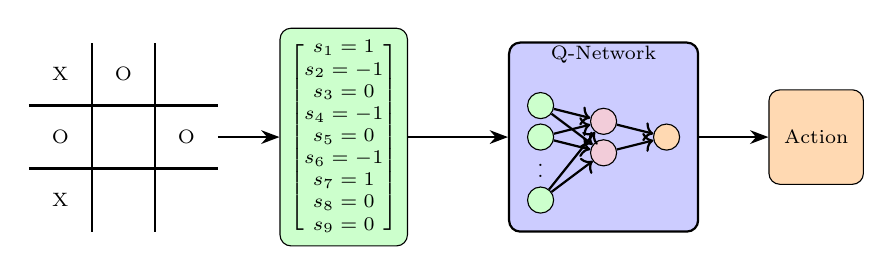
\begin{tikzpicture}[
        qnet/.style={draw, rounded corners, fill=blue!20, minimum width=1.2cm, minimum height=1.2cm},
        module/.style={draw, rounded corners, fill=purple!20, minimum width=1.2cm, minimum height=1.2cm},
        action/.style={draw, rounded corners, fill=orange!30, minimum width=1.2cm, minimum height=1.2cm},
        state/.style={draw, rounded corners, fill=green!20, minimum width=1.2cm, minimum height=1.2cm},
        arrow/.style={->, thick, >=Stealth},
        every node/.style={font=\scriptsize}
      ]
        % Vertical lines
        \draw[thick] (0.8,0) -- (0.8,2.4);
        \draw[thick] (1.6,0) -- (1.6,2.4);
        % Horizontal lines
        \draw[thick] (0,0.8) -- (2.4,0.8);
        \draw[thick] (0,1.6) -- (2.4,1.6);
        
        % Xs and Os
        \node at (0.4, 2) {X};
        \node at (1.2, 2) {O};
        \node at (2, 2) {};
        \node at (0.4, 1.2) {O};
        \node at (1.2, 1.2) {};
        \node at (2, 1.2) {O};
        \node at (0.4, 0.4) {X};
        \node at (1.2, 0.4) {};
        \node at (2, 0.4) {};

        \node[state] (state) at (4,1.2) {
            $\begin{bmatrix}
            s_1 = 1 \\ s_2 = -1 \\ s_3 = 0 \\ s_4 = -1 \\ s_5 = 0 \\ s_6 = -1 \\ s_7 = 1 \\ s_8 = 0 \\ s_9 = 0
            \end{bmatrix}$
        };
        \draw[arrow] (2.4,1.2) -- (state);

        \begin{scope}[shift={(6.5, 2)}]
            % Box and title
            \node[draw, rounded corners, thick, fill=blue!20, fit={(0, -1.6) (1.6, 0)}, inner sep=0.4cm, label={[yshift=-0.4cm]above:Q-Network}] (box) {};
            
            % Input layer
            \foreach \i in {1, 2} {
                \node[circle, draw, fill=green!20, minimum size=0.3cm] (input\i) at (0, -\i*0.4) {};
            }
            \node at (0, -1.2) {$\vdots$};
            \node[circle, draw, fill=green!20, minimum size=0.3cm] (input3) at (0, -1.6) {};
            
            % Hidden layer
            \foreach \i in {1, 2} {
                \node[circle, draw, fill=purple!20, minimum size=0.3cm] (hidden\i) at (0.8, -\i*0.4-0.2) {};
            }
            
            % Output layer
            \node[circle, draw, fill=orange!30, minimum size=0.3cm] (output) at (1.6, -0.8) {};
            
            % Connections
            \foreach \i in {1, 2, 3} {
                \foreach \j in {1, 2} {
                    \draw[->, thick] (input\i) -- (hidden\j);
                }
            }
            \foreach \i in {1, 2} {
                \draw[->, thick] (hidden\i) -- (output);
            }
        \end{scope}
        \draw[arrow] (state) -- (box);

        \node[action] (action) at (10, 1.2) {Action};

        \draw[arrow] (box) -- (action);
        
    \end{tikzpicture}
    \caption{Illustration of a Q-Network processing a Tic-Tac-Toe board state.}
    \label{fig:qnetwork_tictactoe}
\end{figure}




\bibliographystyle{IEEEtran}
\bibliography{references}  % Assuming your .bib file is named references.bib


\end{document}



